% !TeX root = ../main.tex
% Add the above to each chapter to make compiling the PDF easier in some editors.

\chapter{Literature Review}\label{chapter:literaturereview}
This chapter provides a comprehensive review of the literature relevant to teleoperation interfaces for autonomous vehicles, focusing on environmental data visualization and perception modification. The review covers various topics, from the fundamentals of autonomous vehicle technology to specific teleoperation concepts and visualization approaches.
\section{Overview of Autonomous Vehicle Technology}

The Society of Automotive Engineers (SAE) International has defined six levels of
driving automation, as shown in figure 2.1 in their J3016 standard, which has become
the industry’s most widely accepted classification system. These levels range from 0
(no automation) to 5 (full automation), providing a clear framework for understanding
the capabilities of autonomous vehicles \cite{sae2021}

\begin{figure}[h]
    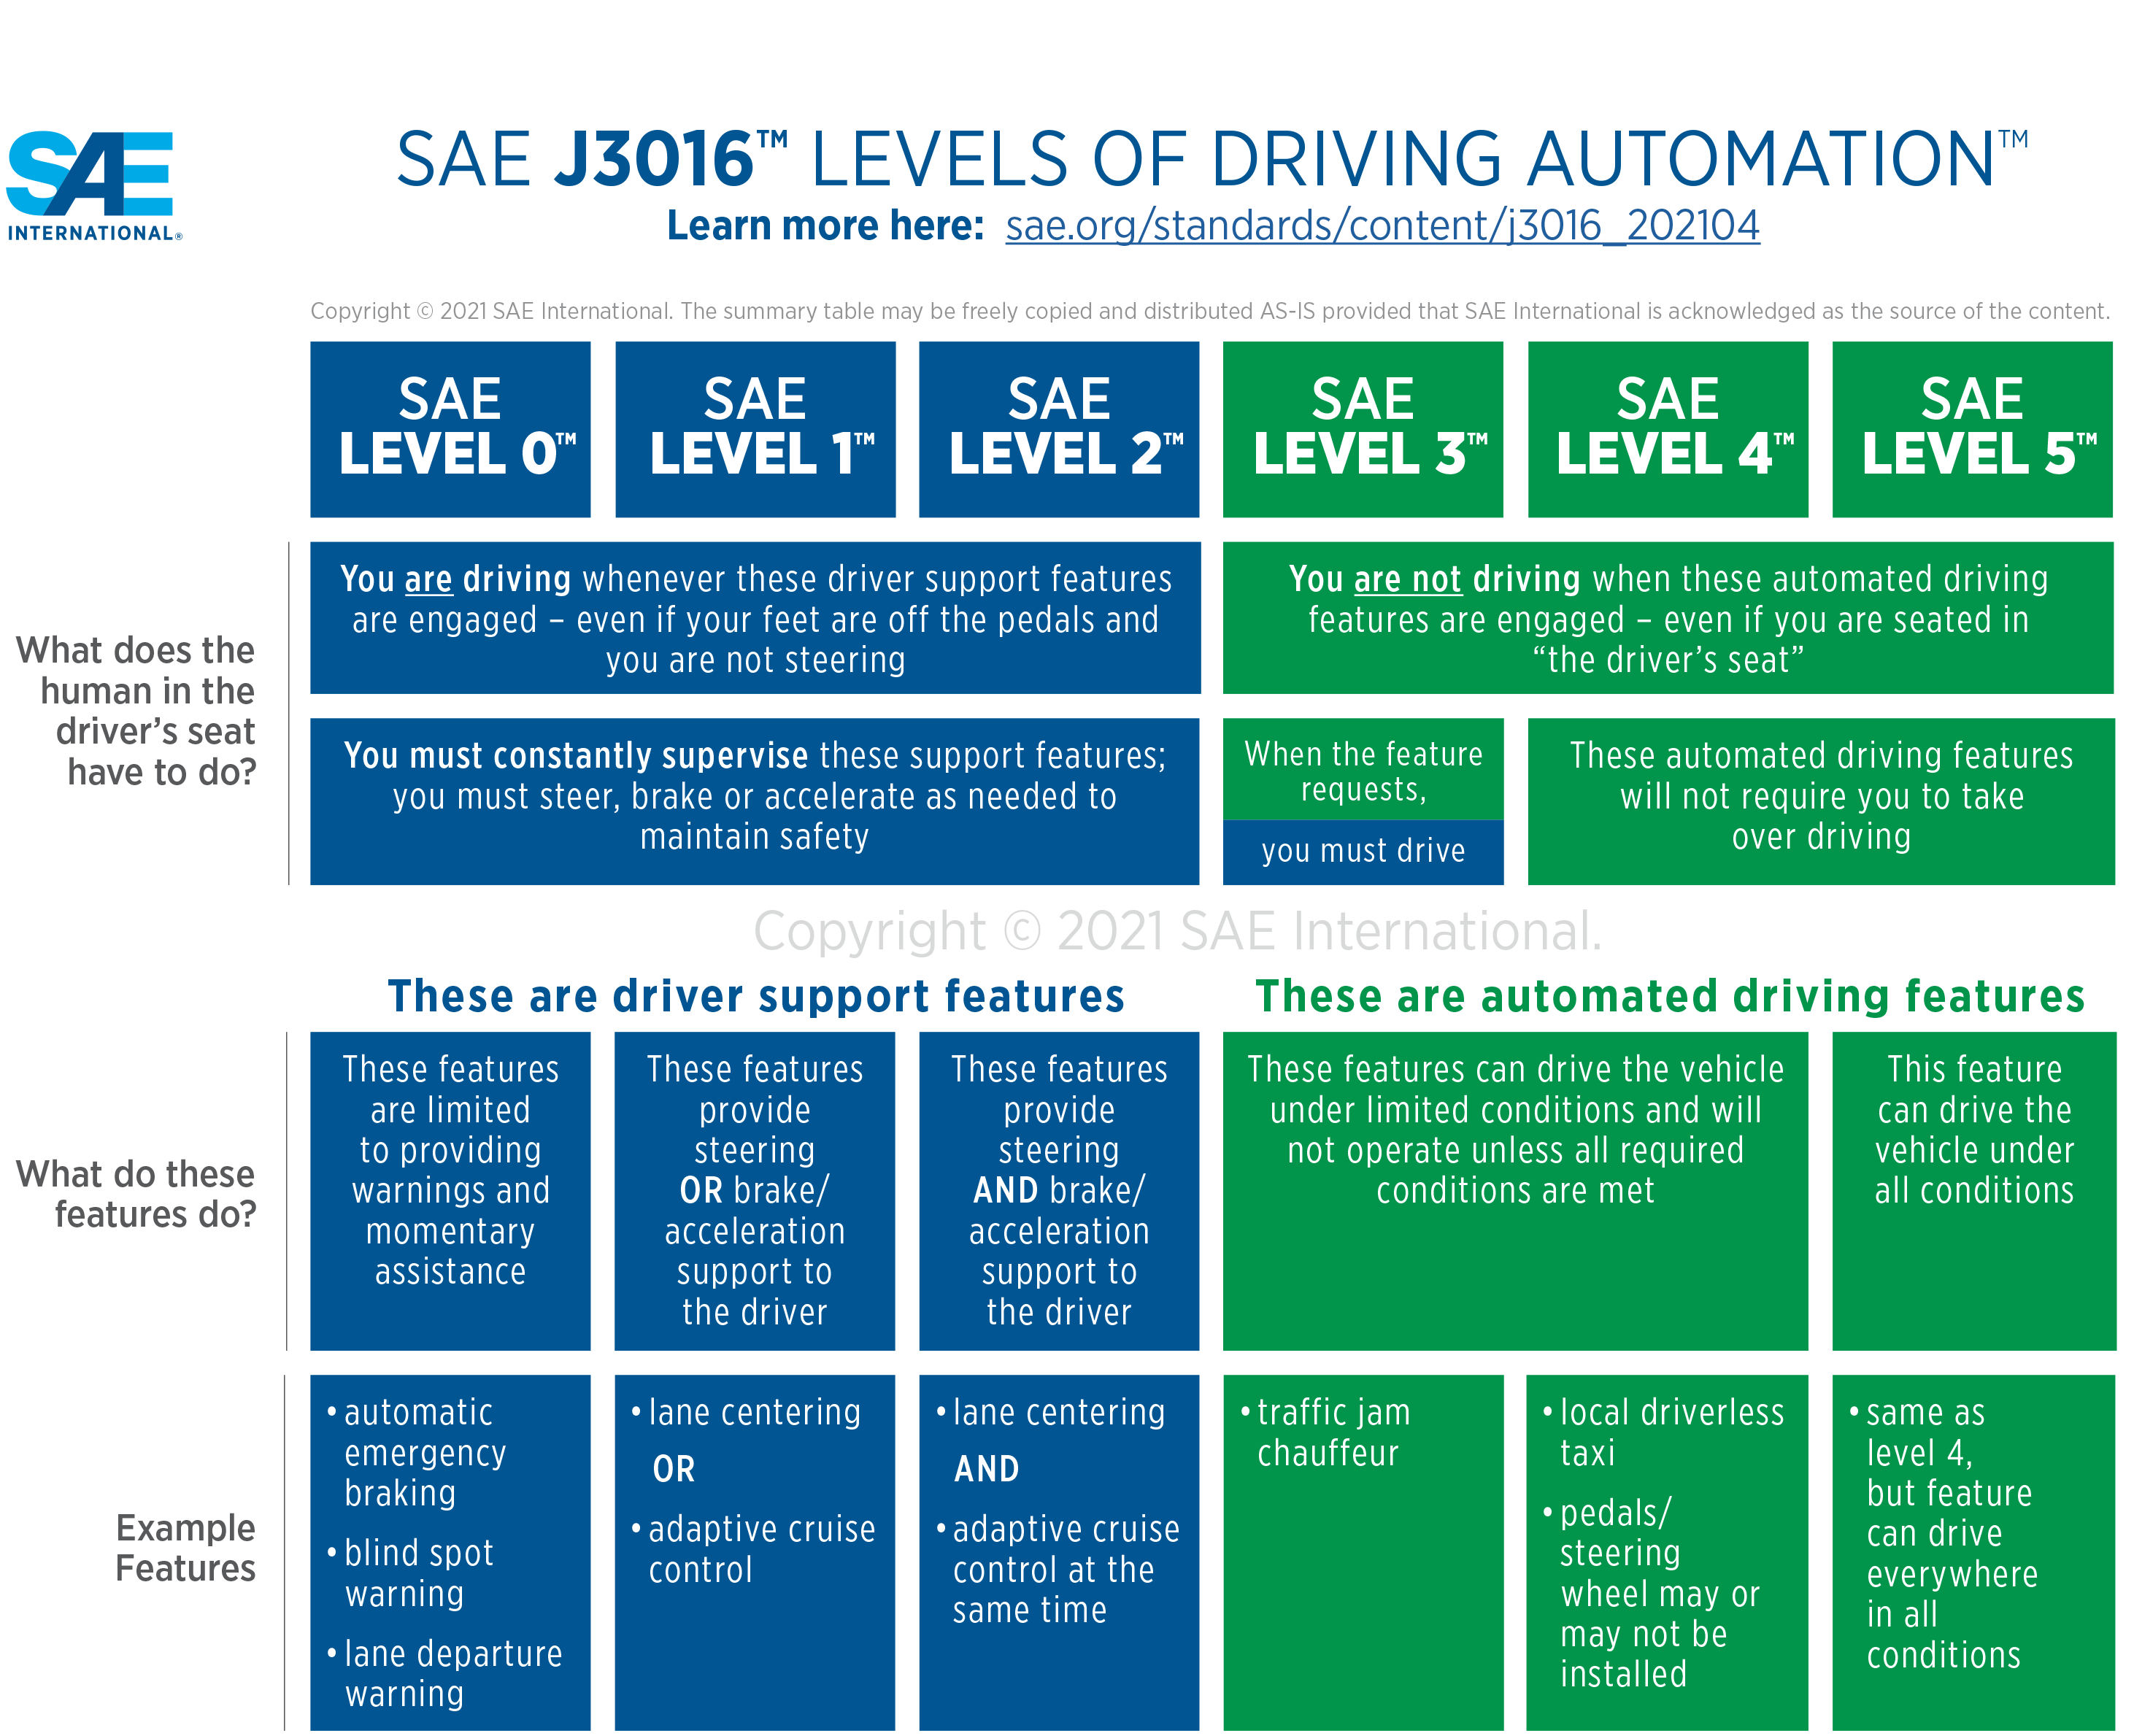
\includegraphics[scale=0.4]{figures/SAE.png}
    \centering
    \caption{SAE Levels of Automation \cite{sae2021}}
    \label{fig:SAE}
\end{figure}

As of 2024, most advanced consumer vehicles operate at Level 2, with some manufacturers pushing towards Level 3 capabilities. For example, BMW has recently become the first carmaker to receive approval for combining both Level 2 and Level 3 autonomous driving systems in a single vehicle. The new BMW 7 Series now offers the BMW Highway Assistant (Level 2) and the BMW Personal Pilot L3 (Level 3), marking a significant step in automated driving technology \cite{bmw2024}.

At the forefront of autonomous vehicle technology, companies like Waymo
are making significant strides towards Level 4 autonomy. Waymo has achieved
Level 4 autonomy in pilot areas, offering fully autonomous rides without safety
 drivers in cities like San Francisco, Phoenix, and Austin \cite{evmagazine2024}.

 Achieving higher SAE levels of autonomy requires a sophisticated autonomous driving stack,
 which is composed of several vital modules that work together to perceive the environment,
 make decisions, and control the vehicle. The stack typically follows a modular software
 architecture that is shown in Figure \ref{fig:AVStack} integrates hardware and software components to enable safe and
 efficient vehicle operation

\begin{figure}[h]
    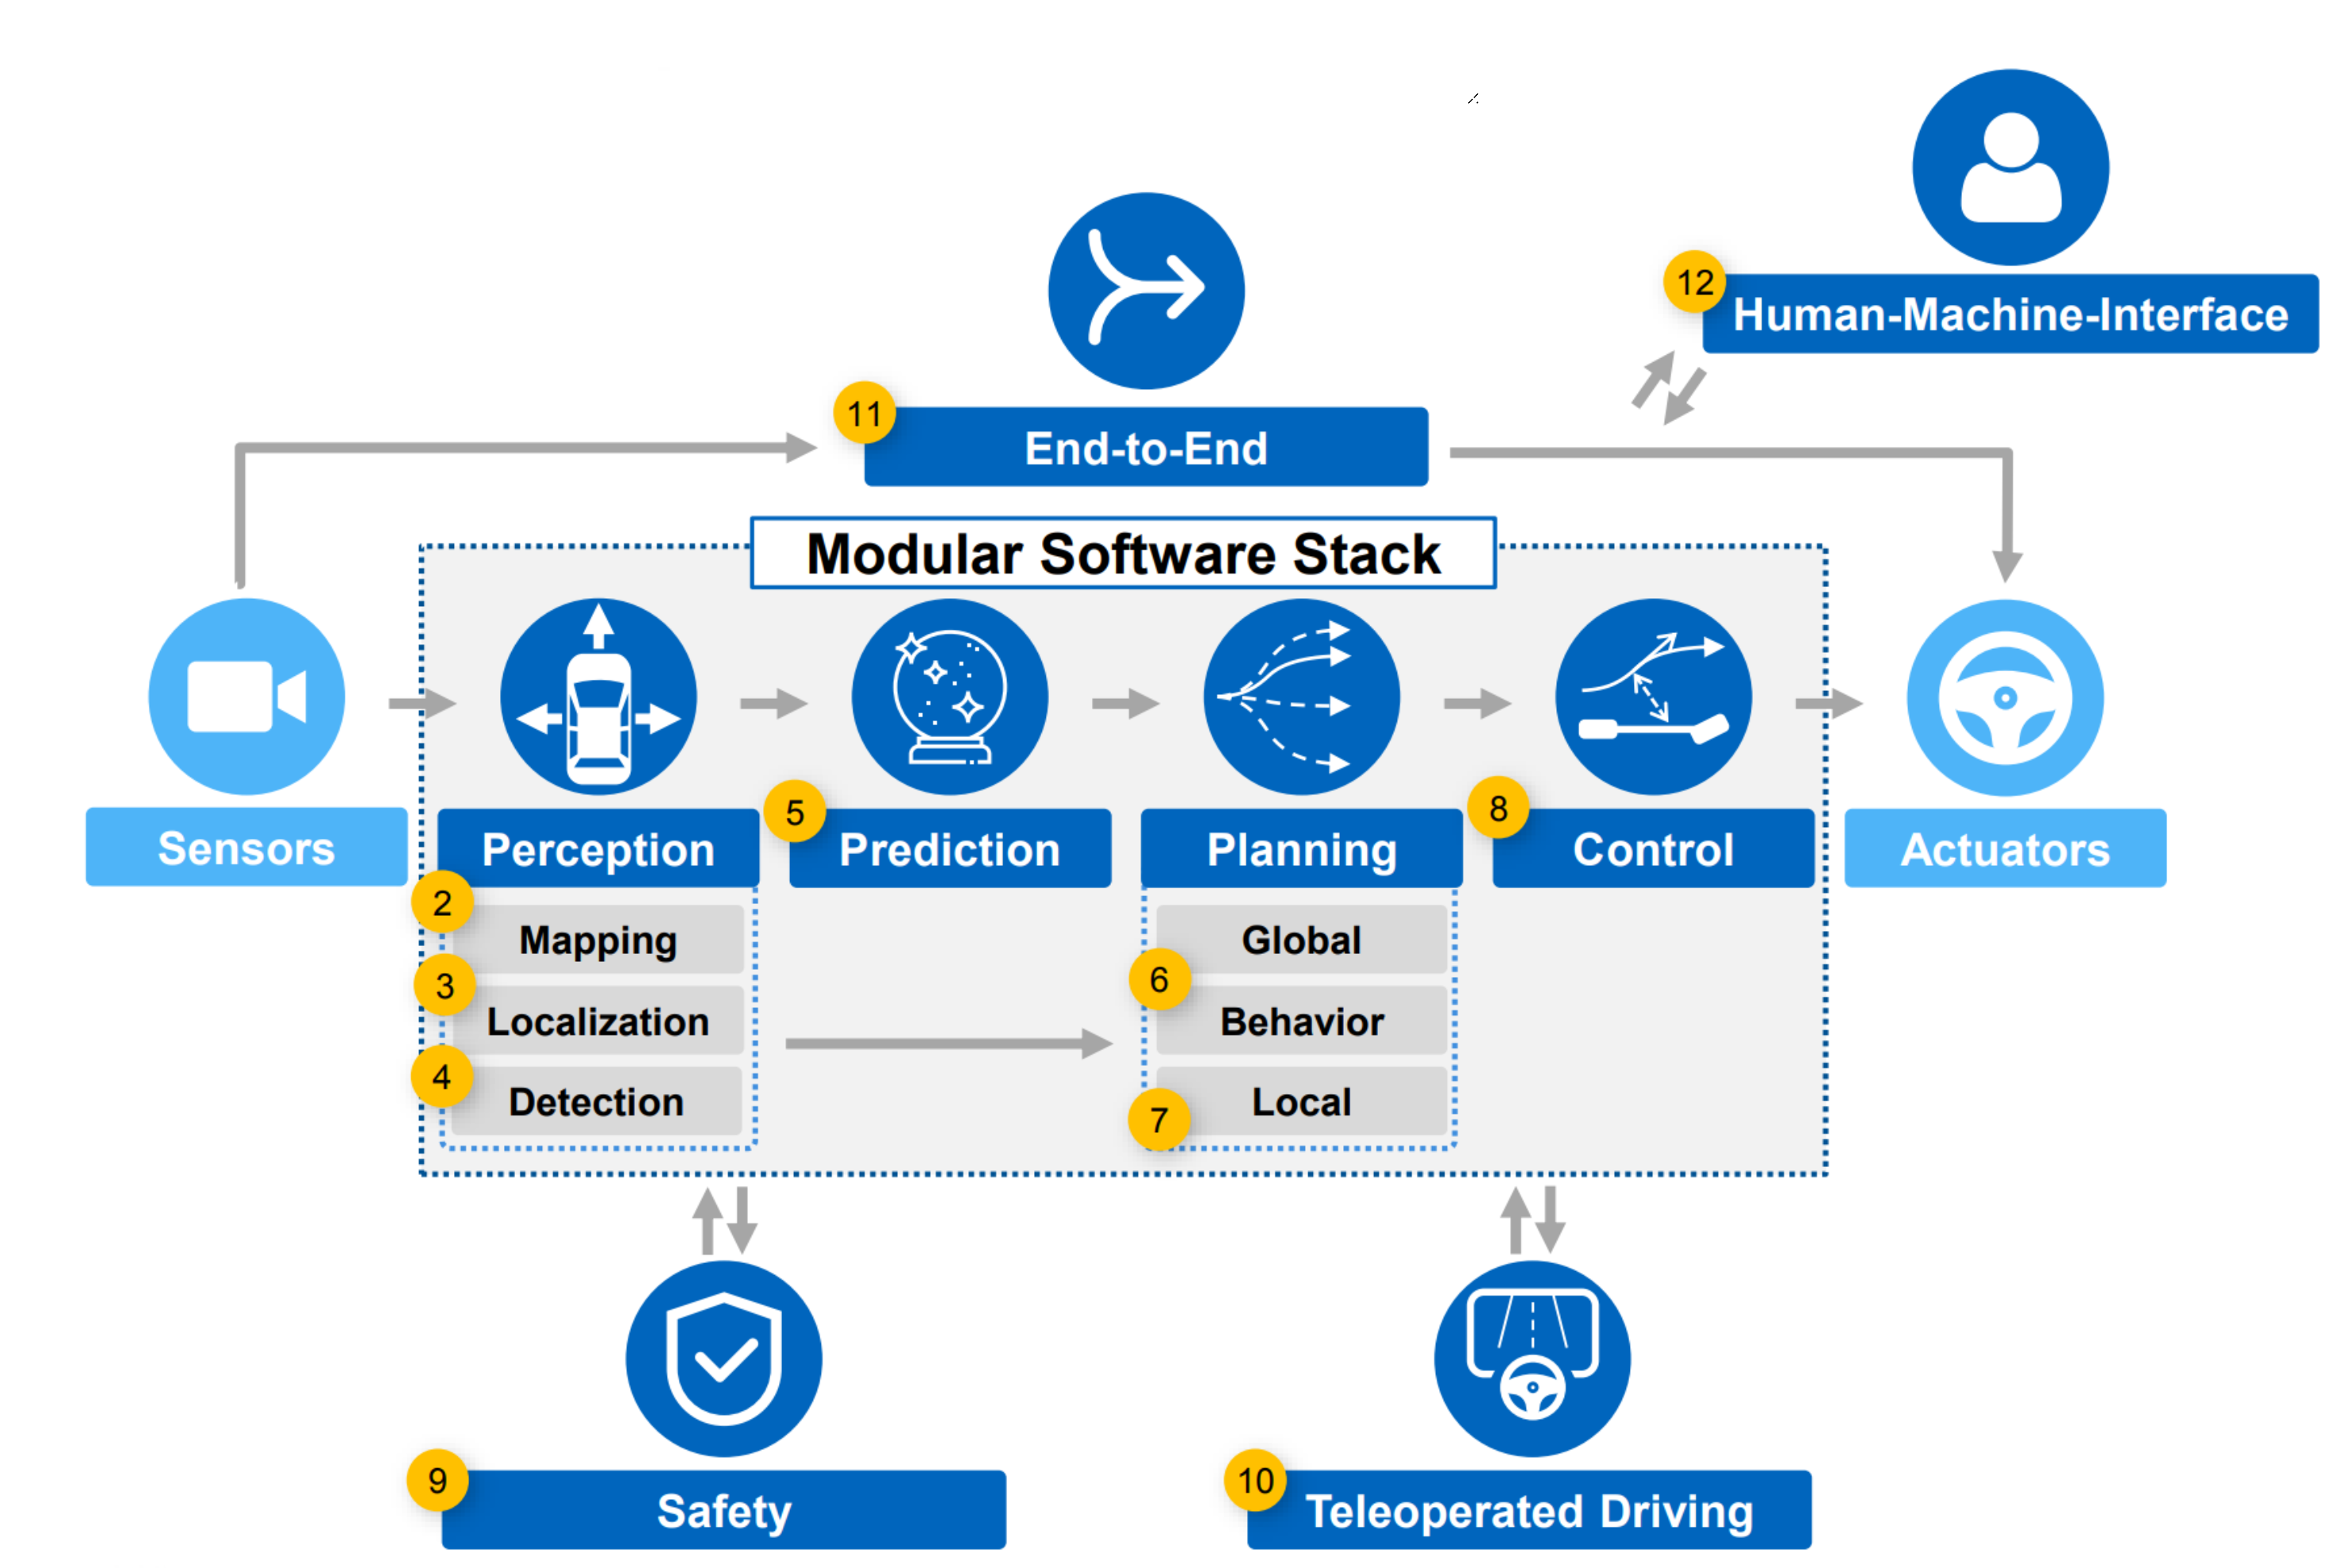
\includegraphics[scale=0.14]{figures/AVStack.png}
    \centering
    \caption{Autonomous Vehicle Technology Stack} %todo: add source from the lecture
    \label{fig:AVStack}
\end{figure}

While some research has explored end-to-end learning, where deep learning models directly map sensor inputs
to control outputs without modular decomposition \cite{codevilla2019limitations}, this approach alone is often
insufficient for achieving higher levels of autonomy. End-to-end systems can struggle with interpretability
and adaptability across diverse driving scenarios \cite{e2e}. It is an active research area and some
of the mentioned issues can be solved with Modular end-to-end learning \cite{nvidia2022diffstack} and also
it is expected to have a better performance on end-to-end methods with the improving hardware and datasets overtime \cite{e2e}.

For a system to reach higher SAE levels—particularly Level 4 or 5—all of
these modules must function reliably across various environments and conditions.
Each component plays a critical role in ensuring that the vehicle can navigate complex urban
environments safely and efficiently while responding to dynamic changes in real-time.
And we have teleoperation for the the cases where one or more module fails to deal the edge cases in the designed level of autonomy.
Teleoperation serves as a bridge between current autonomous driving capabilities and fully autonomous operation.
It allows vehicles to complete their missions even when their onboard systems encounter limitations.
For instance, if an autonomous vehicle encounters a situation outside its Operational Design Domain (ODD)\cite{iso34503},
such as unclear road markings or interactions with law enforcement, it can pull over safely and request human
intervention through teleoperation. This technology is essential for ensuring that autonomous vehicles
can operate reliably in real-world conditions and is expected to play a key role in the widespread adoption of autonomous vehicles.


\subsection{Types of Sensor Data in Autonomous Vehicles} \label{subsection:sensors}
Autonomous vehicles rely on a range of sensors to perceive their environment and
gather the necessary data for safe and efficient navigation. These sensors provide
raw data that is processed by the vehicle's perception system to understand its
surroundings, detect obstacles, and make real-time decisions.
In the later sections we will refer these unprocessed data as "Raw data" or "Raw sensory data".
The key types of sensor data used in autonomous vehicles include:
\begin{itemize}
    \item \textbf{LiDAR (Light Detection and Ranging):}
    LiDAR sensors use laser pulses to measure distances between the vehicle and surrounding objects.
    By emitting laser beams and measuring the time it takes for them to reflect back, LiDAR creates
    a detailed 3D map of the environment. This technology is particularly useful for detecting objects'
    shapes, sizes, and positions with high accuracy, even in low-light conditions \cite{levinson2011towards}.
    LiDAR is widely used in autonomous vehicle systems due to its precision in mapping the surrounding area.

    \item \textbf{Radar}:
    Radar sensors use radio waves to detect objects and measure their speed and distance from the vehicle.
    Unlike LiDAR, radar is less affected by adverse weather conditions such as rain or fog, making it a
    reliable sensor for detecting moving objects like other vehicles or pedestrians \cite{patole2017automotive}.
    Radar is often used for functions like adaptive cruise control and collision avoidance.
    \item \textbf{Cameras}:
    Cameras capture visual data from the environment, providing rich information about road signs,
    lane markings, traffic lights, and other vehicles. Autonomous vehicles typically use multiple cameras positioned
    around the vehicle to achieve a 360-degree view \cite{geiger2012we}. Cameras are crucial for tasks requiring
    high-resolution visual data, such as object classification and scene understanding.
    \item \textbf{Ultrasonic Sensors}:
    Ultrasonic sensors are commonly used for short-range detection tasks like parking assistance or detecting nearby
    obstacles at low speeds. These sensors emit sound waves and measure their reflections to detect objects within
    a few meters of the vehicle \cite{zhang2018ultrasonic}.
    \item \textbf{GPS (Global Positioning System)}:
    GPS provides location data by triangulating signals from satellites. While GPS alone may not offer the precision
    required for autonomous driving, it is often combined with other localization methods such as SLAM
    (Simultaneous Localization and Mapping) to improve accuracy \cite{thrun2005slam}.
    \item \textbf{IMU (Inertial Measurement Unit)}:
    The IMU measures the vehicle's acceleration and angular velocity using accelerometers and gyroscopes.
    This data helps track the vehicle's movement and orientation in real time, contributing to accurate
    localization when combined with GPS data \cite{madgwick2011imu}.
\end{itemize}

We referenced a subset of TUM's EDGAR research vehicle's sensor setup as our basis.
EDGAR is equipped with 10 camera sensors, 4 LIDAR sensors (long and short-range), 6 RADAR sensors as well as GPS, IMU (Inertial Measurement Unit) and microphones \cite{tum2023edgar}

\subsection{Perception Systems in Autonomous Vehicles}
Perception systems are an essential component of autonomous vehicles, responsible for interpreting the
vehicle's surroundings and enabling safe navigation. These systems process data from sensors such as LiDAR,
radar, and cameras to detect and classify objects, track their movements, and localize the vehicle within
its environment \cite{liu2018perception}. The perception system builds a comprehensive model of the environment,
which is then used by other modules—such as prediction, planning, and control—to make driving decisions.

This thesis will refer to "Perception Data" as the processed output from the vehicle's perception system. This includes information about detected objects (e.g., vehicles, pedestrians), their classifications, positions, and trajectories. The perception system also generates high-level semantic information such as lane markings, traffic signs, and road boundaries. This data enables autonomous vehicles to understand their environment and make informed decisions.

We utilize Autoware, an open-source software stack designed for autonomous driving systems for all perception-related tasks in this project. Autoware provides a comprehensive set of tools for processing sensor data and generating perception outputs \cite{kato2018autoware}. It includes object detection, classification, tracking, and localization modules using sensors such as LiDAR, radar, and cameras. By leveraging Autoware's robust perception capabilities, we ensure that our system can handle complex environments while maintaining flexibility for future improvements.

Autoware also supports sensor fusion techniques that combine data from multiple sensors to improve accuracy and reliability. This is especially important when dealing with noisy or incomplete sensor data. For instance, Autoware's fusion algorithms can combine LiDAR point clouds with radar measurements to enhance object detection
performance in adverse weather conditions where cameras may struggle.
\section{Teleoperation Concepts}

Teleoperation is an essential fallback solution for autonomous vehicles (AVs),
enabling a human operator to remotely assist or take control of a vehicle when
its automated systems encounter situations beyond their operational design domain (ODD)
or face disengagements. These scenarios often arise due to complex or unforeseen edge cases,
such as sensor malfunctions, unanticipated obstacles, or ambiguous road conditions.
ensuring that it can resume its mission safely and efficiently \cite{Brecht}.

Several teleoperation concepts have been developed to address different aspects of remote vehicle control, each with its own strengths and limitations. These concepts can be broadly categorized into Remote Driving, Remote Assistance, and Perception Modification. Each approach targets specific challenges in teleoperation, such as latency, situational awareness, and operator workload.

\subsection{Remote Driving}
Remote Driving is one of the earliest teleoperation concepts,
where a human operator takes full control of the vehicle's
dynamic driving tasks (DDT), including steering, acceleration,
and braking. This concept has been explored for more than two decades.
Early research by Sworder et al. \cite{sworder1999performance} (1999) demonstrated the feasibility
of teleoperating vehicles using direct control methods, where
operators manually control vehicles based on live video feeds and
sensor data transmitted from the vehicle to a remote station.
This method, known as Direct Control, has been widely studied
and implemented in various industries since then.

Despite its long history, Direct Control remains relevant
today due to its simplicity and directness. In this approach,
the operator receives real-time video and sensor data from the
vehicle and sends back control commands such as steering angles
or velocity adjustments. However, this method is highly sensitive
to network conditions—particularly latency and bandwidth
limitations—which can lead to reduced situational awareness for
the operator and delayed reactions to dynamic situations \cite{Gnatzig}.
Latency is a critical factor in teleoperation; studies have shown
that latencies greater than 10 milliseconds can result in degraded
performance in high-speed or complex environments \cite{chucholowski2014teleoperated}.
Under fluctuating network conditions—such as handovers
between cellular towers or signal degradation due to obstacles—latency
can increase unpredictably, leading to delayed responses that
compromise safety \cite{neumeier2023feasibility}.

In recent years, several companies have implemented Direct Control
in real-world applications despite these challenges. For example,
Fernride, a Munich-based company, has successfully deployed
teleoperation technology for logistics operations. Fernride's
platform allows remote operators to control semi-autonomous
trucks in logistics yards using Direct Control methods.
In their pilot project with DB Schenker and KAMAG,
teleoperators remotely controlled trucks for yard shunting
tasks—moving trailers around loading docks—demonstrating that
teleoperation can be safely integrated into existing logistics
processes \cite{fernride2023}. The success of this project
highlights the potential of Direct Control in controlled
environments like logistics yards where network conditions are stable.

However, while Direct Control has proven effective in specific use cases
such as logistics yards or industrial environments with
controlled network conditions, it faces significant challenges when
applied to more complex or dynamic environments like urban roads.
The sensitivity of Direct Control to network latency makes it less
suitable for scenarios where real-time decision-making is critical for
safety. To mitigate these challenges, modern teleoperation systems
often incorporate additional safety measures or alternative methods
that reduce reliance on real-time control inputs.

One such alternative is Shared Control, where the vehicle retains
some level of autonomy while the operator provides high-level
inputs. In this approach, if an operator's input does not meet
certain safety criteria—such as proximity to other vehicles—the
vehicle's onboard systems can override those commands to prevent
collisions \cite{kay2024sharedcontrol}. This approach reduces
cognitive load on the operator while ensuring that safety-critical
decisions are still handled by the vehicle's autonomous systems.

\subsection{Remote Assistance}
Remote Assistance focuses on providing high-level guidance or support
to specific functions of the AV without taking full control of the DDT.
This method is often used in scenarios where the AV encounters an
edge case that prevents it from continuing its mission autonomously
but does not require complete human intervention.

In Waypoint Guidance, for example, operators provide waypoints or general
directions for the vehicle to follow while leaving detailed path planning
and execution to the AV's onboard systems \cite{corridor}. This reduces
operator workload but may lead to stop-and-go behavior if communication
between the operator and vehicle is not seamless.

Another promising approach is Collaborative Planning, where operators
work with the AV's planning system by selecting from a set of pre-generated
path suggestions based on sensor data. This method allows operators to focus
on decision-making rather than low-level control tasks \cite{hosseini2024collaborative}.
Collaborative planning improves efficiency but requires robust sensor fusion and reliable
perception data from the AV.
\subsection{Perception Modification}

Perception Modification is one of the most promising teleoperation
concepts, designed to address situations where an autonomous
vehicle (AV) encounters perception errors that prevent it
from continuing its mission. These errors may arise from false
positives or misclassifications in the vehicle's perception system,
such as detecting an object that is not truly obstructing the path or
misinterpreting environmental features like lane markings or road signs.
In such cases, Perception Modification allows a remote operator to
intervene by modifying how the AV interprets its environment,
enabling it to resume its journey \cite{feiler2023perception}.

In this concept, the operator has access to both raw sensor data
(e.g., LiDAR point clouds or camera images) and processed perception
data (e.g., object classifications or environmental models).
By reviewing this data, operators can identify discrepancies
between what the vehicle perceives and what is present in its
surroundings. For example, if a false-positive detection is blocking
the vehicle's path—such as a plastic bag being detected as a solid
obstacle—the operator can modify or correct these perceptions by
marking the area as drivable. This correction enables the AV to
continue its mission without requiring complete manual control \cite{feiler2023perception}.

The Perception Modification concept is beneficial because
it reduces the cognitive load on the operator compared to direct control methods.
Instead of managing all aspects of driving, operators focus solely on correcting
specific perception errors. This approach allows for more efficient human
intervention while minimizing the risk of operator fatigue or error due to
high mental workload \cite{Brecht}. Additionally, Perception Modification can
be extended beyond object detection corrections; operators could also modify other
aspects of the environmental model, such as lane boundaries or drivable space predictions.

As Feiler, et al. \cite{feiler2023perception} define it, the implementation of
Perception Modification involves integrating a  Human-Machine Interface (HMI) that provides operators with real-time access to both raw sensor data and processed perception data. The HMI allows operators to
mark areas as drivable or ignore specific detections deemed irrelevant or incorrect. The vehicle's planning module receives this modified perception data and generates a new trajectory based on these corrections.

In their comparative study of teleoperation concepts, Brecht et al. \cite{Brecht} found
that Perception Modification imposes less cognitive load on operators than
Direct Control while still enabling efficient resolution of disengagements.
The study also highlighted that Perception Modification is highly effective in
situations where false-positive detections or indeterminate objects hinder an AV's progress.
However, it may not be suitable for all disengagement scenarios—particularly those
involving complex trajectory planning failures or situations requiring immediate manual intervention.

\section{Environmental Data Visualization for Autonomous Vehicles}
Environmental data visualization plays a fundamental role in autonomous vehicle systems,
particularly in teleoperation scenarios where human operators must understand and interpret
complex sensor data to make critical decisions.
Visualizing environmental data is crucial for two reasons: First, it enables operators to
maintain high situational awareness during
teleoperation tasks \cite{Gnatzig}. Second, it allows for effective monitoring and verification
of the vehicle's perception system, essential for identifying and correcting potential errors
in the automated driving system \cite{feiler2023perception}.

\subsection{Challenges in Visualizing Multi-Sensor Data}
One of the primary challenges in environmental data visualization is integrating data from multiple
sensors into a cohesive representation of the environment. Modern autonomous vehicles generate
massive amounts of data - up to 3-6 TB of raw data per hour of operation from their sensor suite \cite{kazhamiaka2021challenges}
. A single 4K camera operating at 30 frames per second can produce
approximately 5.4 TB per hour, while a typical AV may have 6-12 cameras along with other sensors \cite{visualcapitalist2024}
. This creates a significant challenge in data processing, transmission,
and visualization. Each sensor type has strengths and limitations, as we defined in section \ref{subsection:sensors}.

The sensor fusion process combines these different data streams into a single, a unified environmental
model that is used by nearly all parts of the autonomous driving stack like perception system \cite{feng2020deep}
, localization system \cite{feng2020deep, el-sheimy2020sensorfusion}. It can also be used for the human operator interface.
However, visualizing this fused data presents several challenges:

\textbf{Real-Time Processing:} Processing and visualizing sensor data in real time requires significant computational resources. Delays in processing can lead to outdated information being presented to the operator, reducing situational awareness \cite{Gnatzig}.

\textbf{Accuracy vs. Latency:} High-fidelity visualizations may improve accuracy but come at the cost of increased latency. A balance between these two factors must be kept for effective teleoperation \cite{chucholowski2014teleoperated}.

Data overload is particularly sensitive in teleoperation scenarios, where operators must quickly understand and respond to complex environmental data while maintaining real-time awareness of the vehicle's situation. This requires careful consideration of which data to present and how to present it effectively without overwhelming the operator's cognitive capabilities.

\subsection{Human Factors in Perception Data Visualization}
We consider two critical elements in teleoperation in the aspect of human factors: situational awareness and mental workload. These factors significantly influence an operator's ability to effectively control and monitor remote vehicles.

\textbf{Situational Awareness:} In teleoperation scenarios, achieving and maintaining situational awareness presents unique challenges due to the physical separation between the operator and the vehicle. Gnatzig et al. \cite{Gnatzig} shows that operators must rely entirely on sensor data and interface representations to understand the remote environment, making the quality and presentation of this information critical for effective operation.  As Endsley \cite{endsley1995toward} states, "Even the
best-trained decision makers will make the wrong decisions if they have inaccurate or incomplete SA.".

\textbf{Mental Overload:} Presenting all sensor data simultaneously can overwhelm operators with too much information.
Operators must process and integrate information from multiple sources while maintaining awareness of critical events, which can lead to increased mental workload \cite{wickens2008multiple}

\section{Existing Approaches to Visualizing Sensor Data}
The visualization of sensor data and perception outputs is crucial for developing and monitoring autonomous vehicles. Various approaches have been developed by both industry and academia to address the challenges of presenting complex environmental data effectively. This section examines existing visualization solutions, starting with industry standards and progressing to more specialized approaches.
\subsection{Industry Standards}
Major autonomous vehicle companies have developed sophisticated operator interfaces to support remote monitoring and intervention when autonomous systems face complex or ambiguous scenarios. These interfaces are designed to provide comprehensive environmental awareness by integrating real-time sensor data, perception outputs,
and vehicle behavior into an accessible format. Below, we highlight examples of operator-focused visualization systems developed by leading companies.

Waymo's Fleet Response Interface \cite{waymo2024fleetresponse}, shown in figure \ref{fig:Waymo} is a prime example of a teleoperation tool designed for remote intervention. This interface provides a detailed 3D visualization of the vehicle’s surroundings, integrating LiDAR point clouds, camera feeds, and object detection data in real-time. Remote operators can monitor the vehicle’s perception system and provide guidance when necessary. For instance, operators can review live video feeds and rewind past footage to better understand complex situations such as construction zones or ambiguous road markings. The system allows operators to suggest lane changes or route adjustments while ensuring the Waymo Driver remains in complete vehicle control.

\begin{figure}
    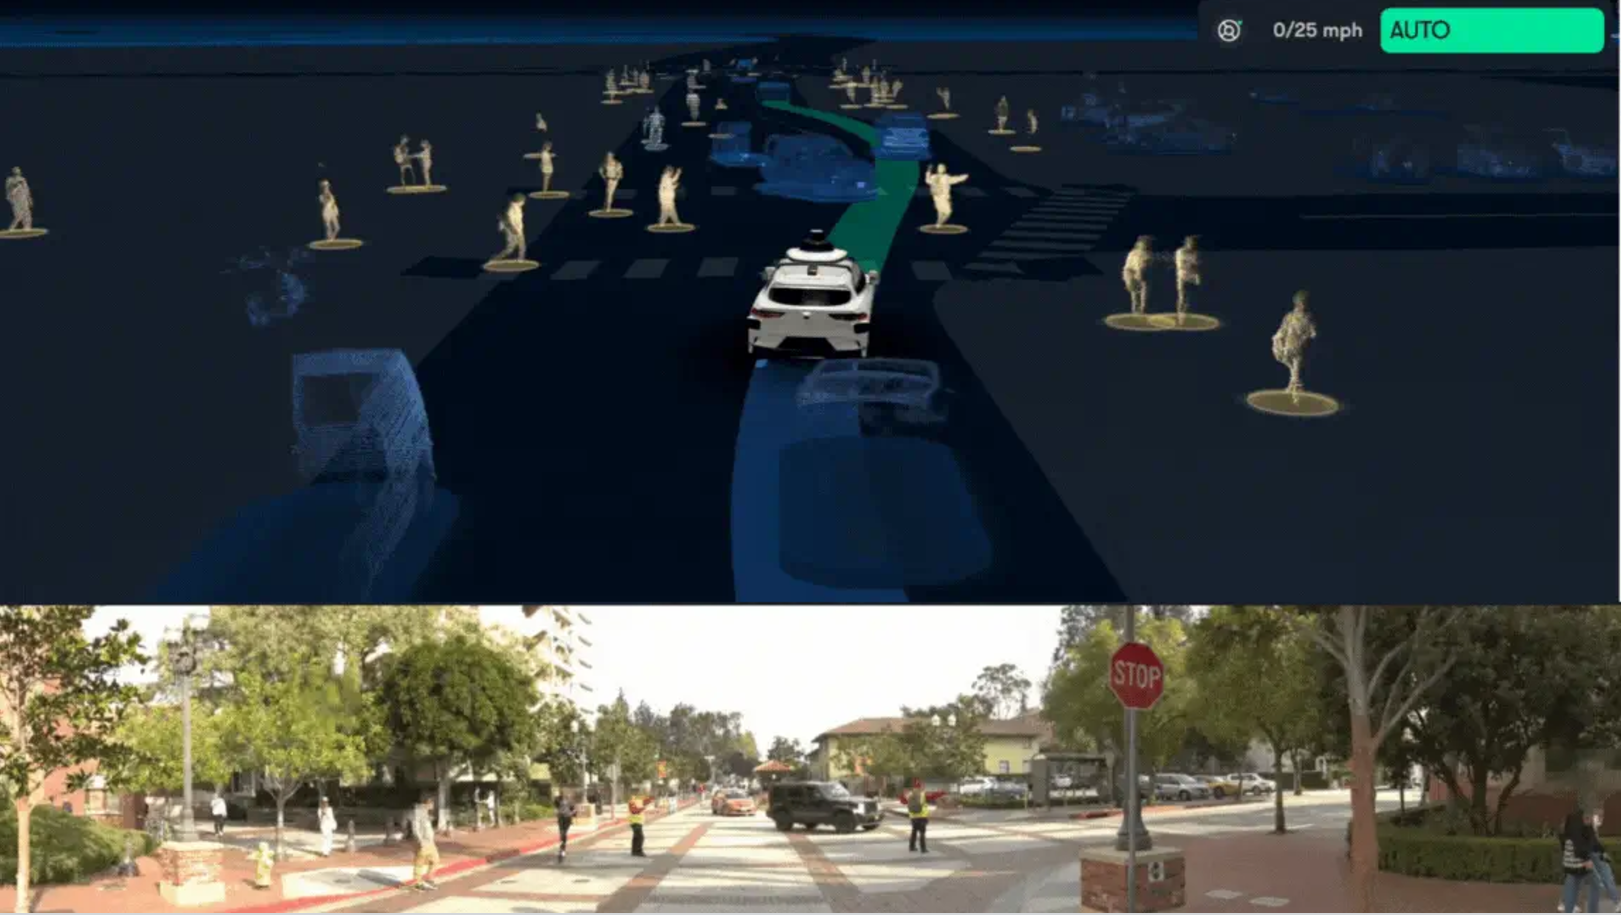
\includegraphics[width=0.8\textwidth]{figures/waymo.png}
    \centering
    \caption{Waymo's Fleet Response Interface \cite{waymo2024fleetresponse}}
    \label{fig:Waymo}
\end{figure}

Zoox's TeleGuidance System \cite{zoox2024teleguidance} is another example of an operator interface designed for remote assistance. Like Waymo’s system, Zoox provides a separate view of the camera feed and a 3D environment model of the vehicle’s perception. This system allows the operator to do both waypoint guidance
 \cite{corridor} and also a subset of perception modification \cite{feiler2023perception} by object recategorization.

\begin{figure}
    \centering
    \begin{subfigure}[b]{0.48\textwidth}
        \centering
        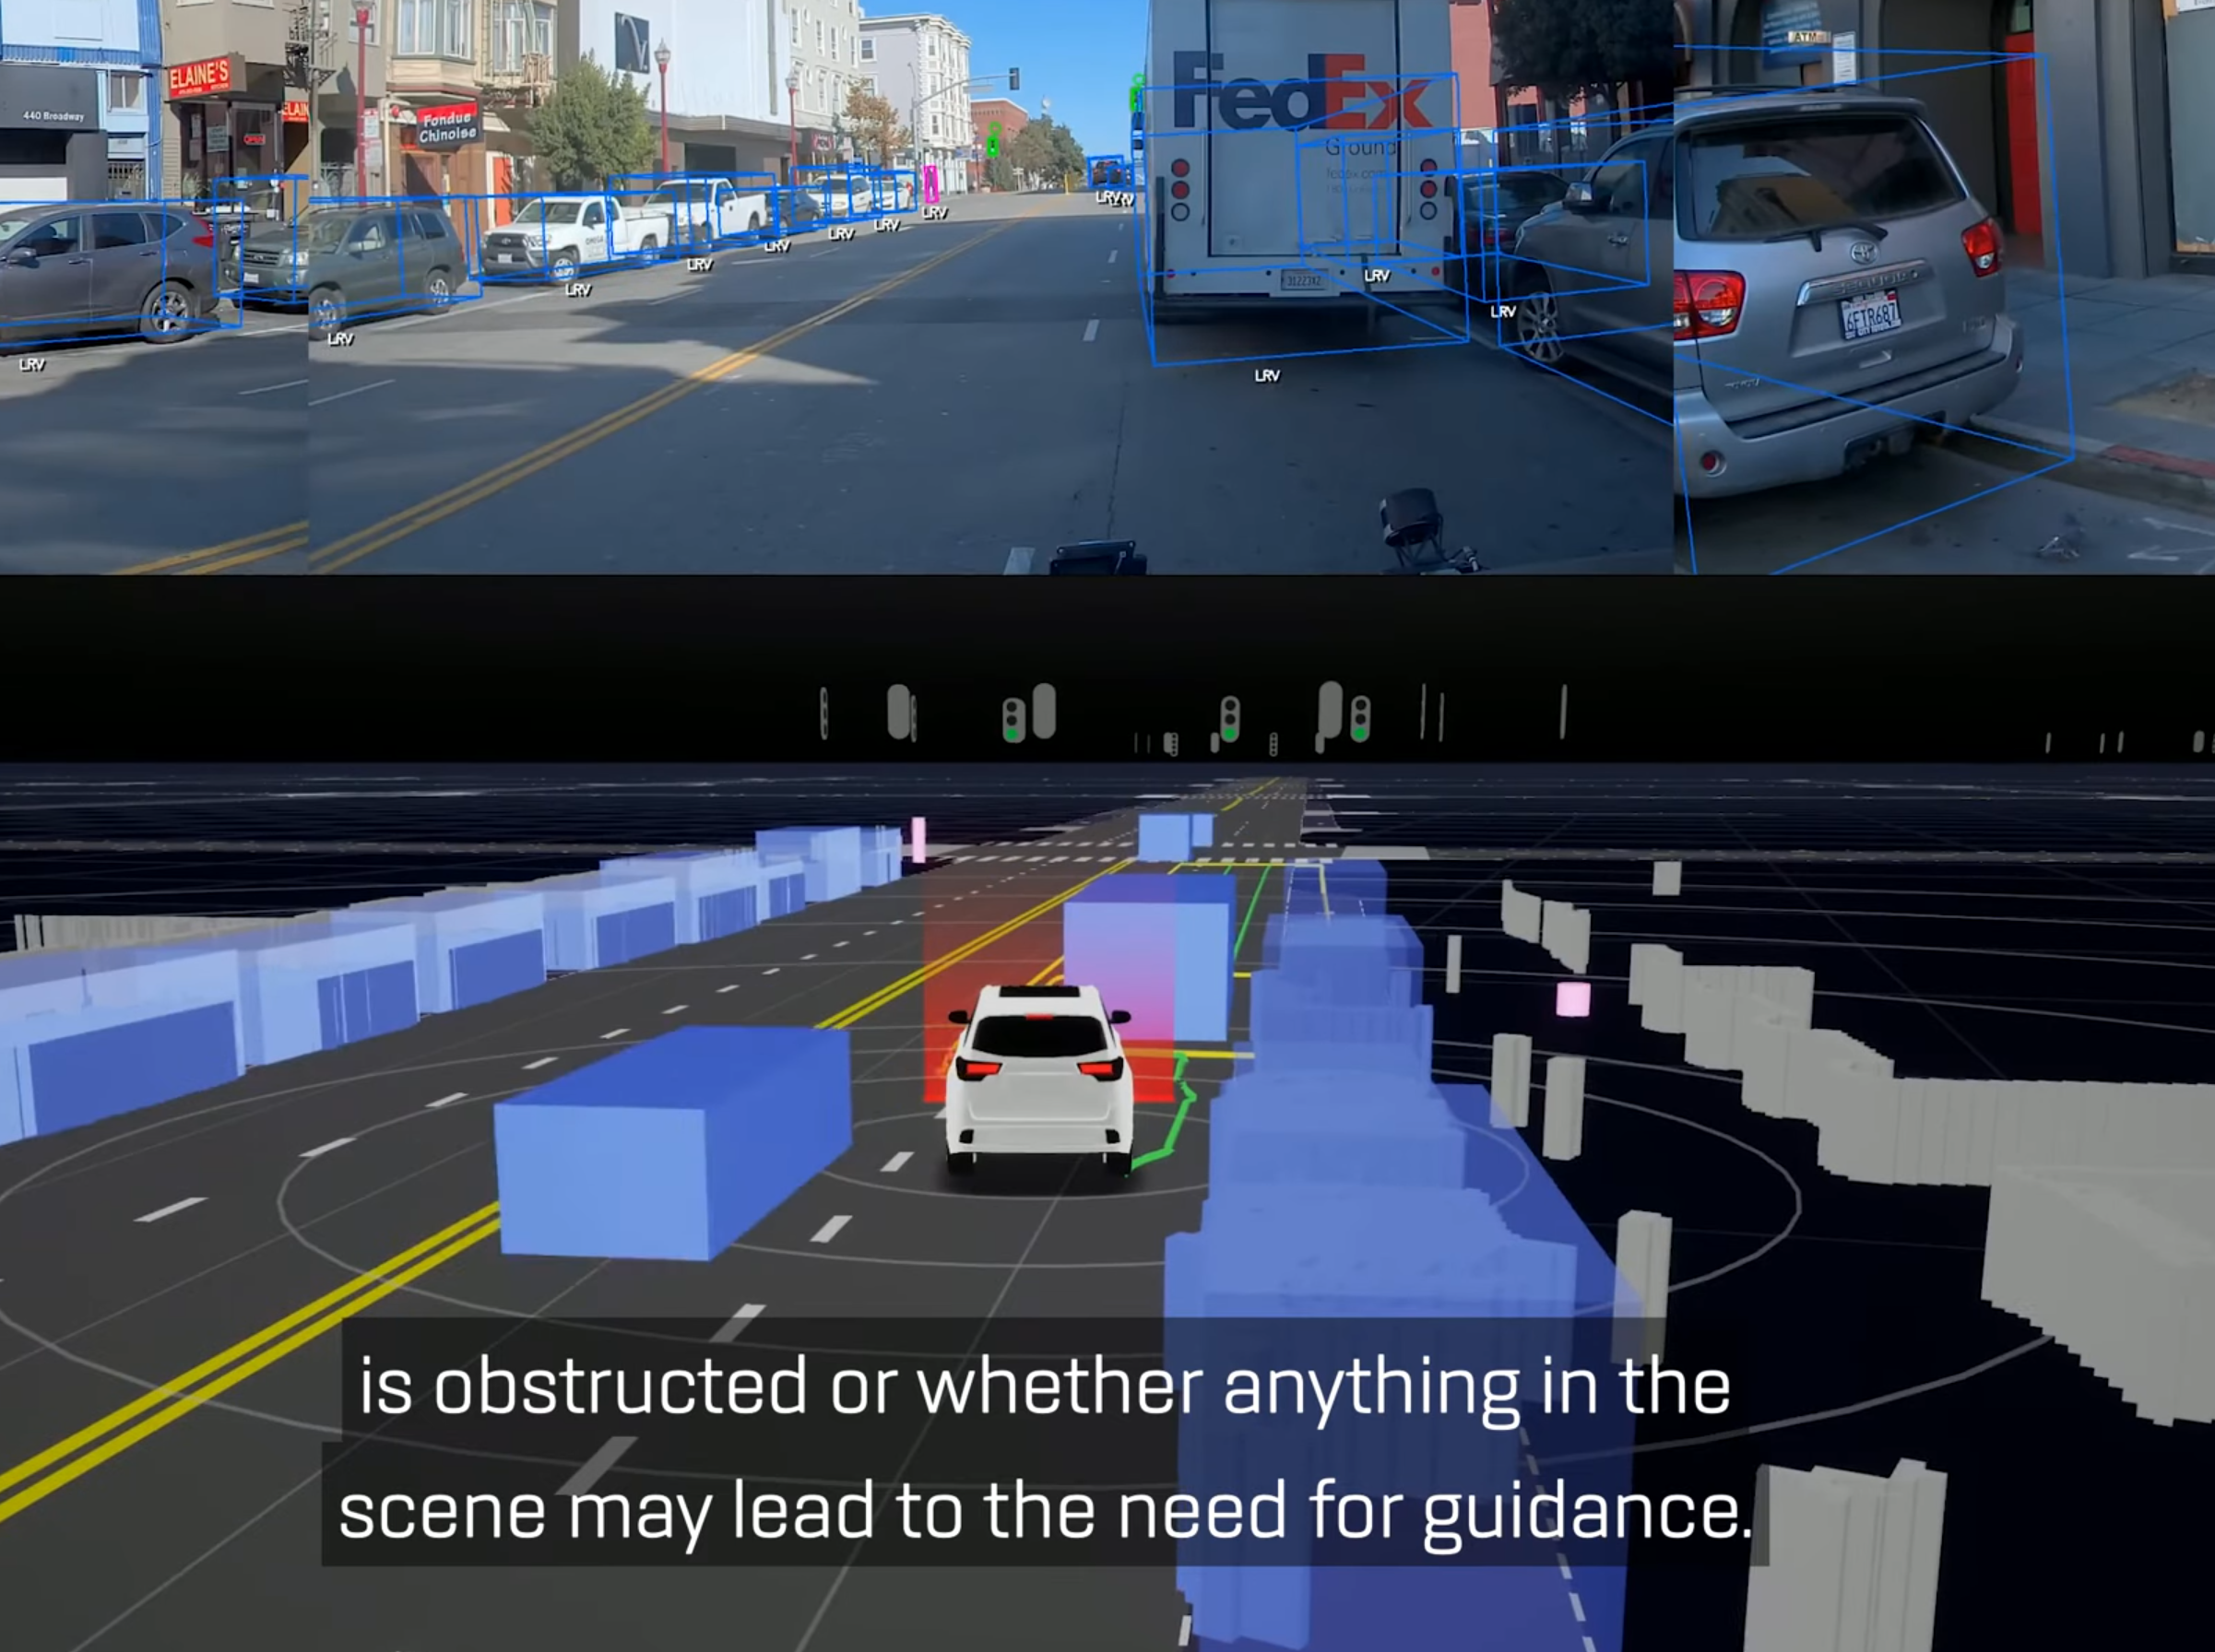
\includegraphics[width=1\textwidth]{figures/zoox.png}
        \caption{Zoox's TeleGuidance System}
        \label{fig:Zoox}
    \end{subfigure}
    \hfill
    \begin{subfigure}[b]{0.48\textwidth}
        \centering
        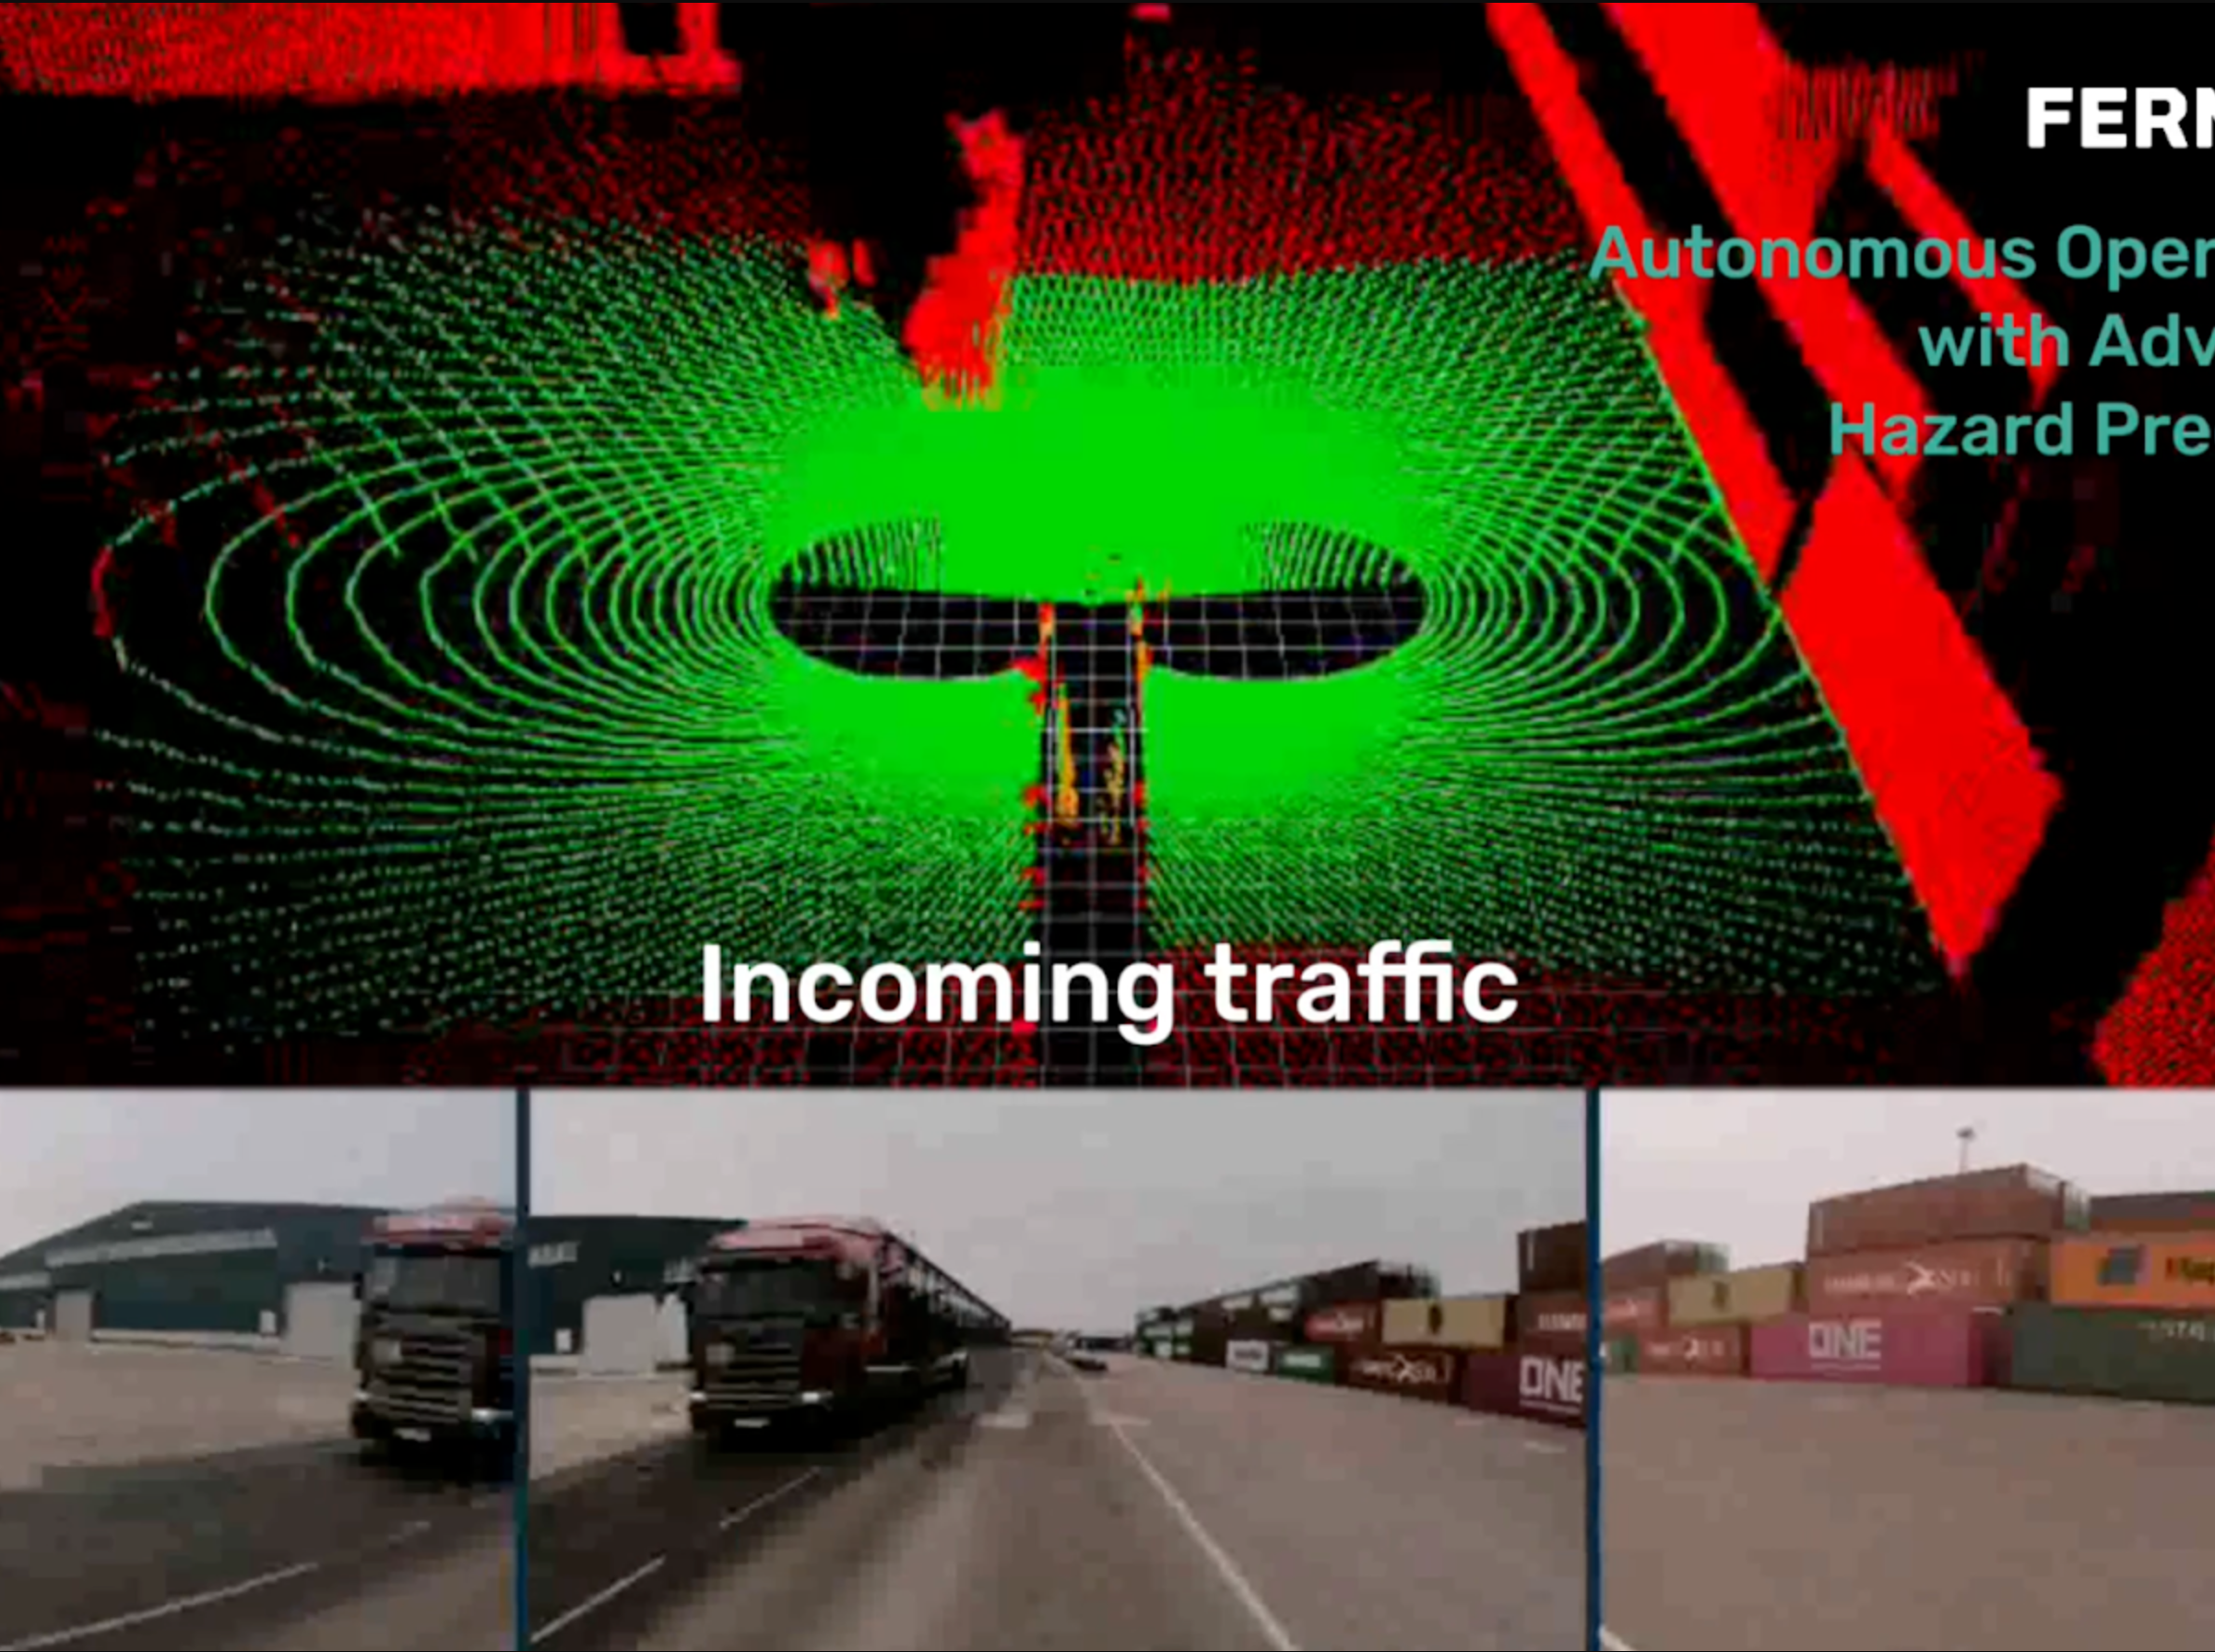
\includegraphics[width=1\textwidth]{figures/fernride.png}
        \caption{Fernride's Teleoperation Interface}
        \label{fig:Fernride}
    \end{subfigure}
    \caption{Comparison of Interfaces for Remote Assistance(a) and Direct Control(b)}
    \label{fig:TeleoperationComparison}
\end{figure}

As shown in \ref{fig:Zoox}, They also provide some perception information mixed in with the video feed.

Fernrides' strategy is different from the other two. They provide a direct
control interface for their teleoperation system. The operator can control the vehicle directly with a joystick and monitor the vehicle's surroundings with a 360-degree camera feed. This approach suits controlled environments like logistics yards, where real-time control is essential for efficient operations \cite{fernride2023}. Since their level of autonomy is lower than that of other examples, the need for perception visualization is also lower. Thus, they focus more on the raw sensory data representations

\subsection{TOD Visual 2.0}\label{subsection:todvisual}
The software stack on which we are building our interfaces is based on TOD Visual 2.0, a teleoperation visualization software developed by the TUM Institute of Automotive Technology. This software is an improved version of TOD Visual \cite{Schimpe}, initially developed for the TUM EDGAR research vehicle. The new version introduces a modular structure, allowing for the easy integration of various visualization approaches and customization to meet specific use cases.TOD Visual 2.0 has already been showcased in public as part of the TUM Wiesn Shuttle event, where it was used to display sensory and perception data during the autonomous shuttle's operation in the challenging traffic conditions surrounding Munich's Oktoberfest \cite{adac2024wiesn, tum2024wiesn}. This real-world demonstration highlighted the software's capabilities in rendering complex sensor data and providing meaningful insights into vehicle behavior under extreme conditions. Although TOD Visual 2.0 is not yet open-sourced, plans are underway to make it publicly available. This will enable broader adoption and collaboration within the research and development community. The software stack provides robust capabilities for rendering sensory information, such as point clouds from LiDAR, camera images, and radar data. Additionally, it supports visualization of perception outputs, including:
\begin{itemize}
    \item Bounding boxes with color-coded classifications for object detection,
    \item Trajectory information for planned vehicle paths,
    \item Lane information derived from offline HD maps.
\end{itemize}

\begin{figure}
    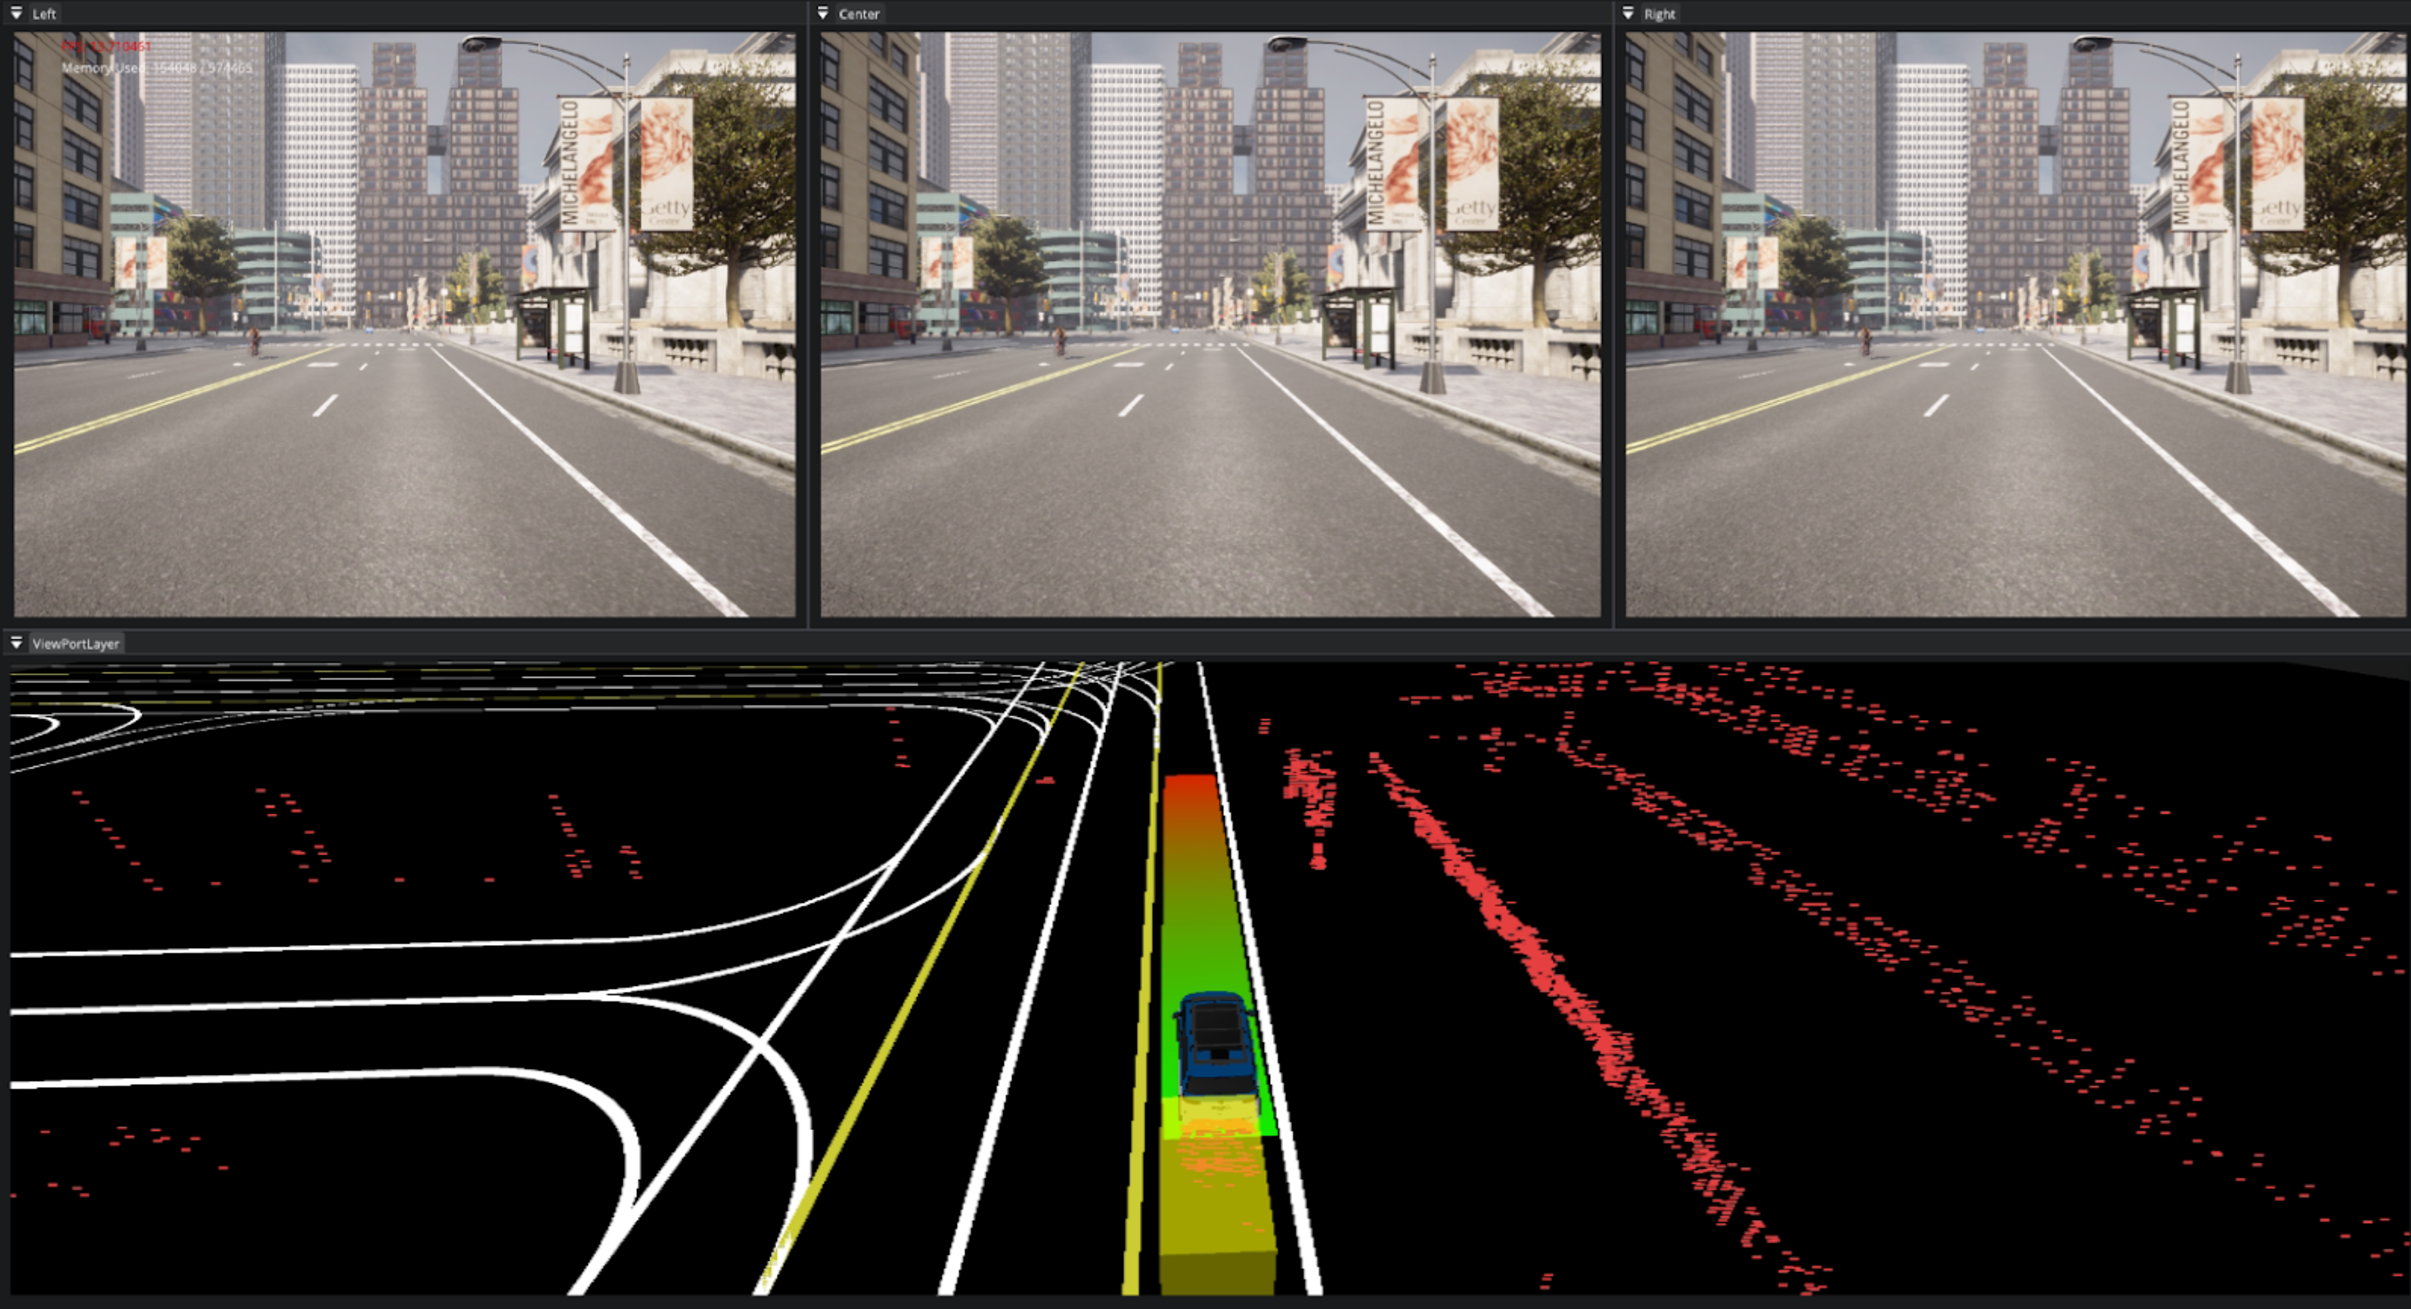
\includegraphics[width=0.8\textwidth]{figures/todvisual.png}
    \centering
    \caption{TOD Visual 2.0 Interface}
    \label{fig:TODVisual}
\end{figure}

The interface before our contribution within this paper can be seen in figure \ref{fig:TODVisual}.

For this thesis, we have taken TOD Visual 2.0 as a foundation and enhanced several components to align with our specific use case. These improvements include refining existing features and adding new functionalities tailored to support our Separate View and Integrated View approaches.


\subsection{Separate View}\label{section:separateview}
In this section, we define the Separate View visualization approach, which involves presenting 2D and 3D data in distinct windows or displays for the operator. This method allows operators to view raw sensor data (e.g., camera images) alongside processed perception outputs (e.g., object detections and classifications) in separate, clearly delineated spaces. By separating these views, operators can compare the raw data against the system's perception outputs to identify potential discrepancies, such as misclassifications or false positives.

The Separate View approach is particularly advantageous for teleoperation scenarios where situational awareness and perception verification are critical. Operators can use the 2D view to observe raw camera feeds for a direct visual understanding of the environment, while the 3D view provides a synthesized representation of the vehicle's perception system, including LiDAR point clouds, object bounding boxes, and trajectory predictions. This dual-view setup aids in identifying errors in the perception system and enables operators to make informed decisions when intervening.
\paragraph{Implementation in Our Work} Our implementation of the Separate View approach builds on a codebase called TOD-Visual 2.0, explained in depth in section \ref{subsection:todvisual}, which provides a foundation for developing advanced teleoperation interfaces.
It gives us the base ability to visualize raw sensor data and special visualizations for some of the perception output.
a parallel thesis project by Yassine El Alami \cite{yassinethesis} focuses on further developing this Separate View concept, exploring ways to optimize its usability and
implementation of visualization methods for required perception components. This collaboration ensures that our work benefits from iterative improvements and shared insights into the challenges and
opportunities associated with this visualization method.

\subsection{Integrated View Approaches}\label{section:integratedview}
We define the Integrated View approach as combining raw sensor data and perception outputs into a
unified visualization for the operator. According to Wickens' multiple resource theory \cite{wickens2008multiple},
humans have limited cognitive resources, and splitting attention across multiple displays can overload these resources,
reducing task performance and situational awareness. The Integrated View aims to mitigate these challenges by
merging raw sensor data with processed perception outputs into a single representation. This approach seeks to enhance
situational awareness and reduce cognitive overload by eliminating the need for operators to manage multiple displays.
However, achieving this integration is not without challenges. A key issue is the dimensionality disparity between the data sources:
visual data from cameras is inherently 2D, while perception data such as LiDAR point clouds exist in 3D.
Ultimately, all this information must be presented to the operator in a 2D format.
This section explores two primary methods for addressing this challenge:
Image Space Representation and 3D Space Representation.

\paragraph{Image Space Representation} One common approach is to project 3D information onto a
2D image space. For example, bounding box projections for object detection are
widely used in autonomous driving systems as can be seen in Zoox's TeleGuidance sytem
on figure \ref{fig:Zoox}. These projections overlay 3D object
detections onto 2D camera images, providing operators with a simplified view of
the environment. Florea et al. \cite{Florea} extend this concept by using semantic segmentation on
3D point cloud data and projecting the results onto 2D images for improved
visualization. Despite its simplicity, this approach has significant limitations.
Critical depth information is lost when 3D data is projected onto a 2D plane. This makes
it difficult to accurately visualize overlays like bounding boxes, trajectories, or
lane markings in terms of their accurate spatial positions. These can be mitigated by
representing them in a way that fits into the perspective view. There are also occlusion
challenges, as the objects closer to the camera may obscure those further away, leading
to incomplete or misleading visualizations.

\begin{figure}
    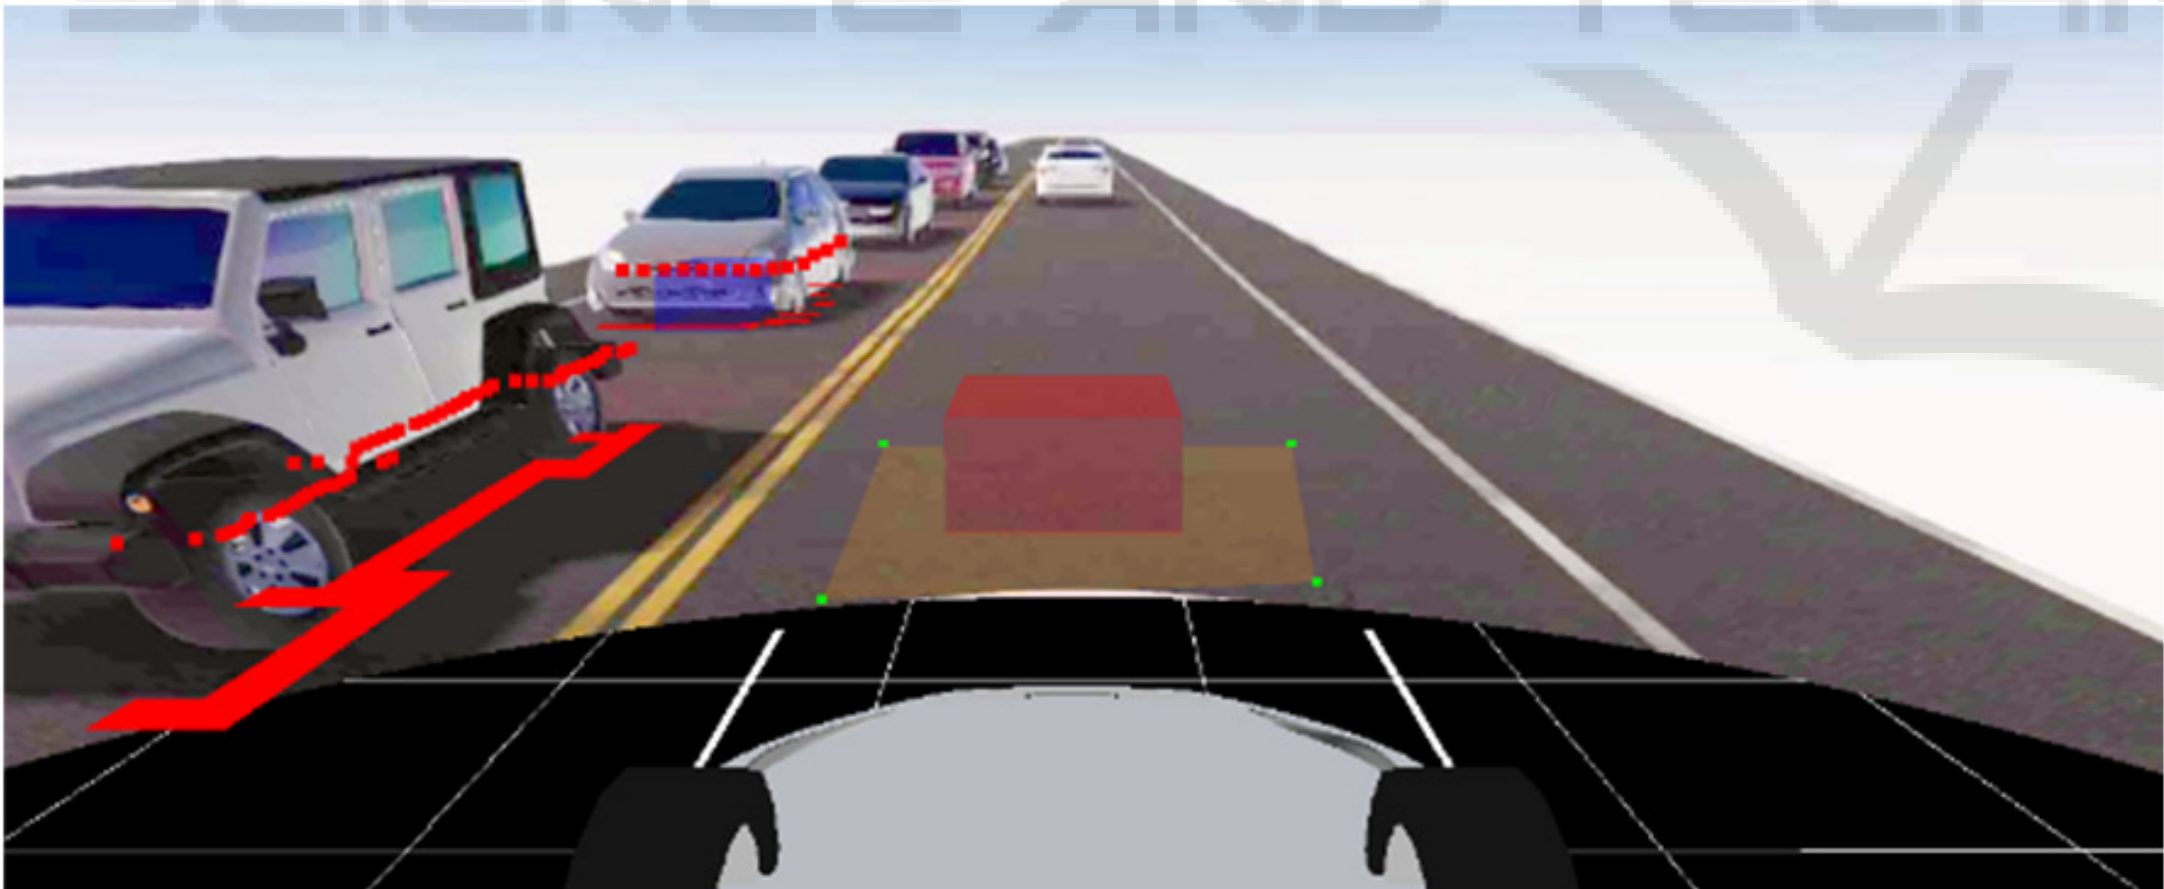
\includegraphics[width=0.8\textwidth]{figures/perceptionMod.png}
    \centering
    \caption{The interface used in the original Perception Modification paper \cite{feiler2023perception}}
    \label{fig:PerceptionMod}
\end{figure}
\paragraph{3D Space Representation} This approach involves maintaining the environmental
data in 3D space while providing methods to integrate 2D camera feeds. This can be
achieved either through projections onto basic geometric shapes, as demonstrated by
Schimpe et al. \cite{Schimpe}, and shown in the figure \ref{fig:PerceptionMod}, or through a comprehensive 3D reconstruction of the surroundings using camera and depth data
. While geometric projection methods offer simplicity, they often encounter issues with collision of perception data points
that do not align with the projected locations. The creation of accurate 3D reconstructions, though more challenging to implement,
provides a more complete and spatially accurate representation of the environment. We will refer to this
comprehensive approach as the "Integrated View" throughout this thesis, as it offers the most promising solution for
combining both raw sensor data and perception outputs in a unified, spatially coherent representation. We will explore
two approaches for implementing this Integrated View. The first approach involves using Neural Radiance Fields (NeRF) to rendering
realistic 3D reconstructions of the environment. The second approach focuses on depth completion techniques to fuse the sensory data
to have a more complete 3D representation of the environment.

\subsection{NeRF-based rendering methods}
Neural Radiance Fields (NeRFs), first introduced by Mildenhall et al. \cite{mildenhall2020nerf}, represent scenes as continuous volumetric functions using neural networks. A NeRF takes a 5D input coordinate (the spatial location $(x,y,z)$ and viewing direction $(\theta,\phi)$) and outputs the volume density and view-dependent emitted radiance at that spatial location. This allows photorealistic novel view synthesis by optimizing the neural network using input images with known camera poses.

In the context of autonomous driving, NeRFs have been particularly effective for static perception tasks such as map construction due to their inherent property of multi-view consistency. Multiple works have applied NeRFs to automotive data, focusing initially on static scenes where the environment remains unchanged \cite{snerf2023}. These approaches typically employ anti-aliased positional embeddings to handle scale variations essential for large-scale scenes.

However, autonomous driving scenarios inherently involve dynamic objects, presenting significant challenges for traditional NeRF approaches. Recent works have proposed methods to handle dynamic scenes to address this limitation. NVIDIA's EmerNeRF introduces a self-supervised approach that decomposes scenes into static, dynamic, and flow fields \cite{yang2023emernerf}. This decomposition emerges from self-supervision, enabling the model to learn from general, in-the-wild data sources without requiring ground truth annotations or external models for dynamic object segmentation.

Similarly, Wayve's PRISM-1 significantly advances handling dynamic urban environments \cite{prism2024wayve}. It can capture complex scenes with multiple moving elements, including pedestrians, cyclists, and other vehicles while accounting for dynamic lighting conditions such as blinking traffic and brake lights. The system learns to separate static from dynamic elements in a self-supervised manner and implicitly tracks movements in the scene, matching them with the 3D geometry.

When considering NeRF-based methods for our Integrated View approach, several factors must be evaluated:

\textbf{Advantages:}
\begin{itemize}
    \item High-fidelity photorealistic reconstructions
    \item Comprehensive representation of both static and dynamic elements
    \item Natural handling of multi-view consistency
\end{itemize}

\textbf{Limitations:}
\begin{itemize}
    \item Significant computational resources are required for training and rendering
    \item Challenges in handling highly dynamic environments with rapid changes
    \item Need for precise camera pose information and multiple viewpoints
\end{itemize}

These characteristics make NeRF-based methods a promising but challenging candidate for real-time teleoperation interfaces. While they offer superior visual quality and spatial consistency, their computational demands and real-time performance limitations must be carefully considered for practical applications. It is important to note that it is a novel approach that has rapidly improved in recent years.

\subsection{Depth Completion}

Depth completion addresses converting sparse and irregular depth data into dense, regular depth information. This process is particularly relevant for autonomous vehicles, where LiDAR sensors provide accurate but sparse 3D measurements. Having complete depth information enables precise scene reconstruction, as the dense depth map allows for accurate projection of camera images onto the 3D space, creating a comprehensive view of the environment\cite{tang2023comprehensive}.

The KITTI depth completion benchmark has become the standard evaluation platform for these methods\cite{uhrig2017sparsity}, providing a dataset of over 93,000 depth maps with corresponding raw LiDAR scans and RGB images. The benchmark evaluates methods using metrics such as iRMSE (inverse root mean square error) and iMAE (inverse mean absolute error) to assess performance against ground truth data.

Recent advances in depth completion have explored various learning approaches. Supervised methods like GuideNet have demonstrated superior performance by effectively fusing image features at different encoder stages with sparse depth features\cite{tang2023guidenet}. The Convolutional Spatial Propagation Network (CSPN) achieves high accuracy with relatively fast runtime, making it suitable for real-time applications\cite{cheng2020cspn}. These supervised approaches, however, heavily rely on ground truth data, which can be costly and challenging to obtain in practical applications.

Self-supervised and unsupervised methods have emerged as promising alternatives that eliminate the dependence on ground truth data. Wong et al. introduced a self-supervised approach that leverages visual inertial odometry to complete depth maps without explicit supervision\cite{wong2020unsupervised}. Recent work by Li et al. explores using 3D perceptual features and multi-view geometry consistency to achieve high-precision depth completion without ground truth data\cite{li2023self}. However, the accuracy remains slightly inferior to supervised methods.

Several factors warrant consideration when considering depth completion for our Integrated View approach. The method provides accurate dense depth information and enables precise 3D scene reconstruction while being computationally more efficient than NeRF-based methods. Some implementations achieve real-time performance, making them suitable for teleoperation applications. However, the approach faces challenges such as dependence on LiDAR sparsity patterns and potential struggles in areas with high occlusion. Additionally, the method requires careful sensor calibration and synchronization to ensure accurate fusion of LiDAR and camera data.

These characteristics make depth completion a promising approach for real-time teleoperation interfaces, mainly when computational efficiency is a priority. Generating dense, accurate depth maps in real time provides a solid foundation for creating comprehensive environmental visualizations for teleoperators.

\section{User Experience and Interface Design for Autonomous Vehicles}
\subsection{Human-Machine Interaction in Autonomous Vehicles}
\subsection{User-Centered Design Principles for Vehicle Interfaces}
\subsection{Cognitive Load and Information Processing in Driving Scenarios}
\subsection{Situational Awareness in Teleoperation}

\section{Evaluation Methods for Visualization Concepts}
\subsection{Usability Testing Techniques}
\subsection{Performance Metrics for Visualization Effectiveness}
\subsection{User Studies in Automotive Interface Design}

\section{Summary}
\subsection{Requirements}
\subsection{Research Gap}


